%!TeX encoding=utf8
\documentclass[ngerman]{scrartcl} 

% Passen Sie hier *Author1*, *Author2* und *Grp.-Nr.* an.
\newcommand{\authA}{Alexander Steding}

\newcommand{\grpnr}{4}
\usepackage{array}
\usepackage{longtable}

% Optionen für die Dokumentenklasse scartcl von KOMAscript. 
\KOMAoptions{
	DIV=11,
	BCOR=0mm,
	paper=a4,
	fontsize=12pt,
	parskip=half,
	twoside=false,
	titlepage=false
}
\usepackage{booktabs}

% Papierformat: DIN-A4, mit wenig Rand 
\usepackage[
	a4paper,
	left=20mm,
	right=20mm,
	top=23mm, 
	bottom=18mm,
	includefoot,
	footskip=8mm
	]{geometry}

% Zeilenabstand, andere Werte: onehalfspacing, doublespacing
\usepackage[singlespacing]{setspace} 

% Definition der Kopf- und Fußzeile
\usepackage[headsepline,automark]{scrlayer-scrpage}
\clearscrheadings
\setlength{\headheight}{2.5\baselineskip}
\setlength{\footheight}{1\baselineskip}
\chead[]{ \\  Abschlussbericht}
\ihead[]{\\ \authA}
\ohead[]{Datum: \today }
\ofoot[]{\pagemark}

%---Language and umlauts
\usepackage[utf8]{inputenc}       % UTF-8 Kodierung - ä, ö, ü, ß direkt eingeben
\usepackage[ngerman]{babel}                      % Neue deutsche Rechtschreibung  
\usepackage[expansion=true, protrusion=true]{microtype} % Bessere Silbentrennung

% Formelsatz
\usepackage{amsmath}		% Mathematik-Umgebungen - z.B. align
\usepackage{amsthm}		% Umgebung "theorem"
\usepackage{amsfonts}	% Schriften
\usepackage{amssymb}		% Symbole
\usepackage{upgreek}		% Griechische Sonderzeichen z.B. \upmu
\usepackage{booktabs}
% Einheiten
\usepackage{siunitx}
\sisetup{
	locale = DE,  
	separate-uncertainty,  
	range-units = brackets,  
	list-units = single,  
	per-mode=fraction
}

% Bilder und Tabellen
\usepackage{graphicx}			% Bilder als PDF einbinden
\usepackage{epstopdf}			% Bilder im EPS-Format
\usepackage{caption}				% Unterschriften für Bilder und Tapellen
\usepackage{booktabs}			% Zusätzliche Schönheitslinien für Tabellen
\usepackage{multirow}			% Mehrere Felder in einer Tabelle zusammenfassen
\usepackage[table]{xcolor}		% Für farbig unterlegte Tabellenzeilen
  \definecolor{lightgray}{gray}{0.9}
  \rowcolors{1}{}{lightgray}	% jede zweite Zeile in einer Tabelle leicht grau


% Positionierung von Bildern und Tabellen
\usepackage{float}				% Option 'H', also "hier-egal-wie-das-aussieht"
\usepackage[section]{placeins}	% Platzierung spätestens am Ende eines Kapitels
\renewcommand{\floatpagefraction}{.75}	% standard: .5
\renewcommand{\textfraction}{.1}			% standard: .2
\renewcommand{\topfraction}{.8}			% standard: .7
\renewcommand{\bottomfraction}{.5}		% standard: .3
\setcounter{topnumber}{3}				% standard: 2
\setcounter{bottomnumber}{2}				% standard: 1
\setcounter{totalnumber}{5}				% standard: 3

\usepackage{caption}
\captionsetup[figure]{name=Abb.}
\captionsetup[table]{name=Tab.}

% Hyperlinks
\usepackage{hyperref}
\hypersetup{
	colorlinks=true, 
	breaklinks=true, 
	citecolor=darkgray, 
	linkcolor=darkgray, 
	menucolor=red, 
	urlcolor=cyan,
	bookmarksopen=false, 
	bookmarksopenlevel=0,
	plainpages=false,			% zur korrekten Erstellung der Bookmarks 
	hypertexnames=false			% zur korrekten Erstellung der Bookmarks 
}

\usepackage{pdfpages} 		% Einfügen von Vollseiten-PDFs (z.B. das Deckblatt)
\usepackage{csquotes}		% Zitate
\usepackage{pythonhighlight}
% Literaturverzeichnis
\usepackage[style=alphabetic,sorting=ynt,backend=biber]{biblatex}

% Eine Abkürzung, die Computerbefehle im Fließtext mit einer Mono-Schrift setzt
% (funktioniert leider nicht für Backslash \ . Da hilft dann der Befehl \verb )
\providecommand*{\code}[1]{{\texttt{#1}}}
\usepackage{listings}
\usepackage{xcolor}

\definecolor{codegreen}{rgb}{0,0.6,0}
\definecolor{codegray}{rgb}{0.5,0.5,0.5}
\definecolor{codepurple}{rgb}{0.58,0,0.82}
\definecolor{backcolour}{rgb}{0.95,0.95,0.92}

\lstdefinestyle{mystyle}{
    backgroundcolor=\color{backcolour},   
    commentstyle=\color{codegreen},
    keywordstyle=\color{magenta},
    numberstyle=\tiny\color{codegray},
    stringstyle=\color{codepurple},
    basicstyle=\ttfamily\footnotesize,
    breakatwhitespace=false,         
    breaklines=true,                 
    captionpos=b,                    
    keepspaces=true,                 
    numbers=left,                    
    numbersep=5pt,                  
    showspaces=false,                
    showstringspaces=false,
    showtabs=false,                  
    tabsize=2
}

\lstset{style=mystyle}
\usepackage{hyperref}
\begin{document}
\shorthandoff{"}           % Anführungszeichen nicht als Befehl interpretieren



\begin{titlepage}
\begin{center}
\vspace{3cm}
{\fontsize{40}{49} \selectfont \textbf{Programierpraktikum Übung 4}}\\[2cm]
\Large{\authA }\\
\Large{10028034 }\\
\large{Gottfried Wilhelm Leibniz Universität\\{\today}}
\end{center}
\end{titlepage}
\stepcounter{page}

\newpage

\section{Übung 1}
\section{Übung 2}
\section{Übung 3}
\section{Übung 4}
\subsection{Vergleichsplot}
Gefragt war in dieser Übung nach einem Vergleich der MonteCarlo Methode und dem Prairie-Grass-Experiment. Zusätlich sollte das MonteCarlo Modell um eine Integration der Prandtlschicht erweitert werden. Eine besondere Herausforderung war zu dem die Integration einer exakten Gitterauswertung. Für die Berechnung der Konzentrationen und das Visualisieren wurde Python verwendet. Dargestellt wurden jeweils die berechnete Konzentrationen mit dem MonteCarlo Modell und die gemessenen Werte aus dem Experiment für verschiedene Höhen.

In dem Praire-Grass-Experiment wurden die Quellstärke nicht weiter konkretisiert, deshalb wurden verschieden Quellstärken ausprobiert. Zunächst mit der Quellstärke

\begin{equation}
Q= 150 \frac{g}{s}
\end{equation}
Dies liefert den folgenden Graphen: 
\begin{figure}[H]
    \centering
    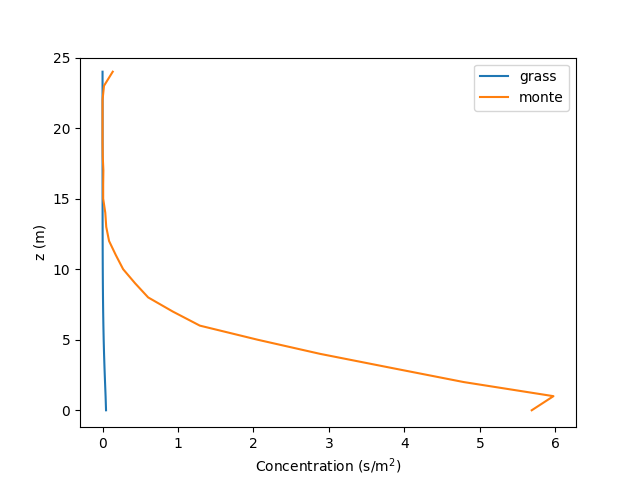
\includegraphics[scale=1]{Bilder/150.png}
    \caption{Vergleich MC und Grass für Q=150}
    \label{fig:my_label}
\end{figure}

Das  MonteCarlo Modell liefert mit diesem Q nur eine sehr schlechte annäherung für Höhen unter 10m.

Ein Q von
\begin{equation}
Q= 0.15 \frac{g}{s}
\end{equation}
 liefert folgenden Graphen:
\begin{figure}[H]
    \centering
    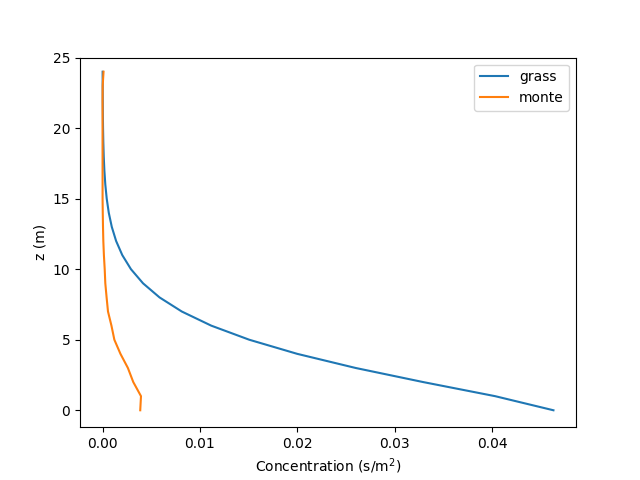
\includegraphics[scale=1]{Bilder/015.png}
    \caption{Vergleich MC und Grass für Q=0.15}
    \label{fig:my_label}
\end{figure}
Diese Quellstärke ist zu gering und das MonteCarlo liefert auch hier nur eine schlechte Anpassung.

Eine Quellstärke von 
\begin{equation}
Q= 1 \frac{g}{s}
\end{equation}
liefert optimale Ergebnisse:
\begin{figure}[H]
    \centering
    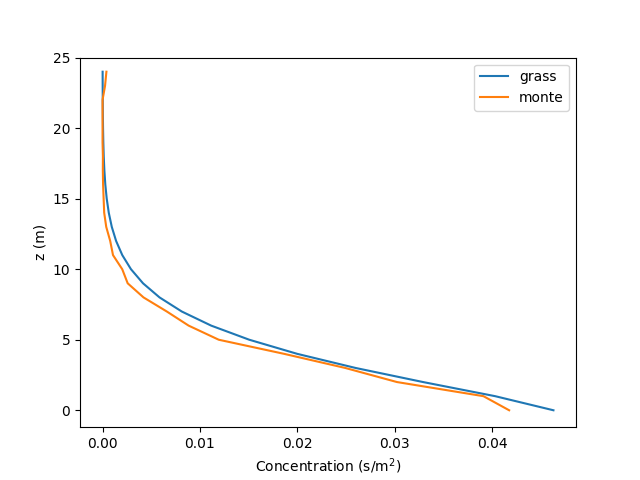
\includegraphics[scale=1]{Bilder/1.png}
    \caption{Vergleich MC und Grass für Q= 1}
    \label{fig:my_label}
\end{figure}

Das MonteCarlo Modell 0schafft hier eine sehr gute Annäherung an das Experiment über alle Höhenbereiche hinweg. Lediglich bei Höhen unter 2m gibt es eine stärkere Abweichung. Dies könnte in der nicht optimierten komplexen Reflexion unter $z_{0}$ liegen, welche in der nächsten Übung in den Ablauf integriert werden kann.


\section{Quellcode}
\subsection{Python}
\subsubsection{Angepasstes MC Modell}
\lstinputlisting[language=Python]{Code/colab.py}
\subsubsection{Darstellung und Vergleich mit dem Grass Experiment}
\lstinputlisting[language=Python]{Code/grassmodul.py}
\end{document}
